\documentclass[tcc, capa]{texucpel}

\usepackage[utf8]{inputenc}
\usepackage[T1]{fontenc}
\usepackage{verbatim}
\usepackage{amsmath}
\usepackage{graphicx} % para inserir figuras

\usepackage{microtype} % detalhes de justificação e espaçamento
\usepackage{nowidow} % evita que a última linha de um parágrafo mude de pag.
\usepackage{paralist} % lista sem o espaçamento de uma linha entre itens
\usepackage{booktabs} % 'rules' em tabelas
\usepackage{multirow} % Mágicas com tabelas
\usepackage{amssymb} % checkmark
\usepackage{icomma} % corrigir decimais (exceto unidades SI)
\usepackage{fourier} % muda a fonte de matemática pra colidir menos com arial
\usepackage{nameref}
\usepackage{verbatim}
 \usepackage{float}
\usepackage{siunitx}

\sisetup{
	detect-family = true,
	detect-shape = true,
	detect-weight = true,
	detect-mode = true,
	output-decimal-marker = {,},
	binary-units = true
}%



\newcommand{\esp}{ESP8266}
\newcommand{\esppci}{ESP-01}
\newcommand{\exehda}{EXEHDA}
\newcommand{\middleware}{\emph{middleware}}
\newcommand{\pic}{PIC}
\newcommand{\picm}{PIC18F4550}
\newcommand{\picf}{PIC18F}
\newcommand{\hc}{HC-05}
\newcommand{\meter}{\mbox{ubiMeter}}

\newcommand{\gambi}{\fontfamily{phv}\fontshape{n}\selectfont}
\newcommand{\media}{\(\textrm{\gambi{} Média (\si{\volt})}\)}
\newcommand{\desvio}{\(\textrm{\gambi{} Desvio Padrão}\)}
\newcommand{\maximo}{\(\textrm{\gambi{} Máximo (\si{\volt})}\)}
\newcommand{\minimo}{\(\textrm{\gambi{} Mínimo (\si{\volt})}\)}
\newcommand{\erromed}{\(\textrm{\gambi{} Erro médio}\)}
\newcommand{\erromax}{\(\textrm{\gambi{} Erro máximo}\)}

\unidade{Centro de Ciências Sociais e Tecnológicas}
\curso{Engenharia de Computação}
\nomecurso{Engenharia de Computação}
\titulocurso{Engenheiro de Computação.}

\title{Otimizando função de pontuação de docking molecular com uso de Florestas Aleatórias}

\author{de Campos}{Gianluca}
\vspace{1.2cm}

\advisor [Prof. Me.]{Mertins}{Luciano Edson}
%\coadvisor [Prof.]{Sobrenome}{Nome}

\keyword{Otimização}
\keyword{Estrutura}
\keyword{Avaliação}

\begin{document}
\maketitle 
\renewcommand{\advisorname}
{Orientador}          
%\renewcommand{\coadvisorname}{Coorientador}      %descomente caso tenhas coorientadora
\sloppy
\fichacatalografica
\folhadeaprovacao
%Opcional
%\begin{dedicatoria}
%\end{dedicatoria}

%Opcional
\begin{agradecimentos}
\textbf{Agradecimentos} \\
Em primeiro lugar gostaria de agradecer ao apoio de meus familiares por ser possível estar aqui estudando nesta instituição, dando o máximo de suporte possível para que eu pudesse estar aqui hoje. Agradeço também aos colegas de turma e trabalho pelo auxílio nas difíceis tarefas no estudo e também pelo monitoramento delas. Agradecimento também ao meu Orientador por se disponibilizar para me ajudar ao longo deste ano para concluir este trabalho.
\vspace{\baselineskip}
\end{agradecimentos}

%Opcional

\begin{epigrafe}{John Lennon}
"When I was 5 years old, my mother always told me that happiness was the key to life. When I went to school, they asked me what I wanted to be when I grew up. I wrote down ‘happy’. They told me I didn’t understand the assignment, and I told them they didn’t understand life."\\
\end{epigrafe}

%Resumo em Português (no máximo 500 palavras)
\begin{comment}
O processo de desenvolvimento de fármacos é normalmente algo custoso financeiramente, que demanda muito tempo e recursos para serem realizados, muitas vezes é feito por uma pessoa de forma manual. 

Esta questão pode ser melhorada, caso todo o processo fosse automatizado computacionalmente, mais especificamente tendo, um software que examine a estrutura de uma célula ligante e também faça a comparação entre suas similaridades com outra célula, esta sendo chamada de receptora, afim de ter um mapeamento de moléculas  que definem  ambas estruturas das  duas células e também a avaliação do quanto estão bem ligadas, para isto é aplicada uma técnica, chamada de Docking Molecular.

Os softwares existentes, utilizam o docking para este processo de avaliação, porém, possuem um precisão de acertos imprecisos ao lidar com grandes volumes de dados para serem avaliados. 
Para que possa ser melhorada a precisão desses softwares, deve ser feito uma otimização na função de avaliação usado nestes softwares e treina-la com deep learning, para que assim o processo de docking esteja trabalhando com melhores resultados. 
\end{comment}

\begin{abstract}
O processo de desenvolvimento de drogas medicinais é demorado,custoso e em grande parte manual.
Para melhorar e condicionar uma droga a um efeito desejado, utiliza-se uma técnica chamada Docking Molecular, que consiste em realizar atracamento de células e substâncias,onde o seu resultado demonstra o quão bem ligadas suas estruturas estão.Este processo é feito em grande parte por softwares, que exibem a melhor opção e combinações no design das células, ainda que estejam bem limitados em sua capacidade de predizer seus resultados.Uma possível solução seria utilizar Redes Neurais para otimizar este processo e diminuir o número de informações necessárias passadas para avaliação.
\end{abstract}

\begin{englishabstract}
  {Titulo do Trabalho em Inglês}
  {Algorithm, Optimization, Evaluation}  
  
The process of developing medicinal drugs is time-consuming, costly and largely manual.
In order to improve and condition a drug to a desired effect, a technique called Docking Molecular is used, which consists of docking of cells and substances, where its result demonstrates how well bound their structures are. \\
This process is largely done by softwares, which display the best choice and combinations in cell design, even though they are quite limited in their ability to predict their results.
A possible solution would be to use Neural Networks to optimize this process and decrease the number of information needed for evaluation.

\end{englishabstract}

%Lista de Figuras
\listoffigures

%Lista de Tabelas
\listoftables

\begin{listofabbrv}{RFCOMM}
		\item[UCPel] \textit{Universidade Cat\'olica de Pelotas}
        \item[CAPRI] \textit{Critical Assessment of PRedicted Interactions}

        
        
\end{listofabbrv}

%Sumario
\tableofcontents

\chapter{Introdução}
Ao ser desenvolvida uma nova droga é necessário estudar as propriedades químicas e analisar a estrutura das moléculas, o processo de desenvolvimento é bem custoso, pois leva tempo para poder realizar testes e avaliar resultados,que são feitos em vitro e examinados em laboratório sendo em grande parte manual e dependente de um ser humano.%\textbf{REF}%CITAR REFERENCIA DE COMO É FEITO DOCKING MANUALMENTE

Por consequência disso é comum que seja utilizado softwares que analizam estruturas celulares e aplicam a técnicas específicas da área de biomedicina, sendo uma delas o docking molecular, que ajuda a simular o comportamento entre duas estruturas ao se juntarem.
Com isto é possível poupar tempo e diminuir o custo de recursos no desenvolvimento de fármacos.

É de conhecimento geral que a tecnologia evoluiu muito nos últimos anos, em especial na computação, tanto no software como no hardware,  em razão disso os programas que realizam docking hoje em dia tem cada vez maior capacidade para processamento, permitindo que seja obtido melhores resultados, desempenho e maior riquezas de detalhes ao explorar uma estrutura celular por exemplo, que pode ser vista de forma tridimensional.

Esses detalhes são importantes para aplicar o docking, pois trazem bastante informação ao realizar o estudo do comportamento entre duas estruturas celulares, que geralmente costumam ser um sequenciamento de DNA ou uma proteína.%\textbf{REF} % citar exemplo

Este comportamento é útil para o desenvolvimento de fármacos, podendo ajudar a estudar inibidores de um vírus por exemplo,  onde ao aplicar a técnica de docking foi possível descobrir substâncias que pudessem inibir o vírus Influenza\cite{ishikawa2011binding}.

A técnica de docking consiste em analisar duas estruturas de células e junta-las com a melhor conformidade de encaixe possível, sendo a partir disto, possível de analisar as propriedades em comum e estuda-las.

Para poder aplicar o docking é necessário conhecer a molécula ligante, qual o receptor que seria qual estrutura ela irá se ligar (proteína ou DNA). Ao conhecer as estruturas, é avaliado qual o melhor ponto em que serão encaixadas e a quantidade de energia que será liberada ao ocorrer esta ligação.

Este processo de avaliação foi calculado através diversos algoritmos ao longo dos anos como; algoritmo genético \cite{holland1975adaptation},  Simullate Annealing \cite{kirkpatrick1984optimization} ,  algoritmo genético de Lamarca \cite{morris1998automated},  MonteCarlo \cite{caflisch1992monte} entre outros que foram tiveram evoluções ao longo dos anos. 

Dependendo do algoritmo utilizado, a precisão do resultado pode variar, assim como seu desempenho e rapidez para gera-lo.
Com a evolução da área computacional, novos estudos são feitos para obter dados com melhor desempenho, em particular a Deep Learning tem se mostrado útil para vários estudos na área de biomedicina conforme avaliado por \cite{korotcov2017comparison,mamoshina2016applications}
, esta técnica basicamente consiste em treinar a máquina, para que ela possa classificar algo em grande escala afim de se obter da melhor forma possível  os resultados.


\section{Objetivo do trabalho}
Tendo em vista que o processo de desenvolvimento de fármacos é custoso, demorado e geralmente necessita de monitoramento, é necessário utilizar algum software que utilize a técnica de docking molecular para automatizar o processo.

O problema é que nem sempre os resultados gerados pela avaliação dos softwares são rápidos e precisos, essencialmente ao avaliar grandes volumes de dados.

Aproveitando a evolução de tecnologia que ocorreu tanto da área da biomedicina e computação, é possível otimizar o processo de docking utilizando técnicas de aprendizado de máquina, em especial, Redes Neurais Profundas (Deep Learning).

Esta mesma classificará da melhor forma a(s) função(ões) de avaliação, ao utilizar estruturas já conhecidas em bases de dados e realizando a comparação.
Dividindo as etapas do docking em processos menores, ajudando a processar um volume de dados maior e também a ter melhores resultados.


\section{Organização do texto}
Neste trabalho foram divididos da seguinte forma.
O Capítulo 2 abrange o referencial teórico sobre o qual será desenvolvido o trabalho de conclusão de curso, em específico, falará sobre a definição do que seria o docking, como é realizado o processo de docking, o contexto de onde está inserido, da mesma forma será feito ao falar sobre a Deep Learning.

No Capítulo 3, é apresentado como será realizado o estudo e otimização na avaliação do docking molecular ao aplicar Deep Learning, contendo uma descrição dos componentes necessários para fazê-la.

\chapter{Fundamentação Teórica}
Este capítulo faz uma breve revisão teórica sobre os assuntos necessários para a entender o processo de docking molecular  e deep learning.

\section{Docking Molecular}
No final da década de 1980, surgiram os primeiros softwares que realizavam o processo de docking molecular, possibilitando desta forma trazer uma visão mais detalhada das estruturas. Com isso foi possível manipular as moléculas e otimizar as células com mais facilidade e simular com maior precisão, permitindo mais rapidez ao realizar testes virtuais.

Para realizar o docking, é necessário realizar o mapeamento das proteínas que irão se ligar, isso serve para prever os melhores pontos para que as moléculas se liguem, e conhecendo assim o ponto com melhor conformidade e energia que será gasta para a união. Isto pode ser visto na figura 1, onde mostra duas protéinas realizando  docking e consequentemente gerando inúmeros pontos de conformidade.

      \begin{figure}[!htb]
	\centering
 \cite{xue2015protein}
    \caption{Exemplo de dockagem entre duas proteínas}
    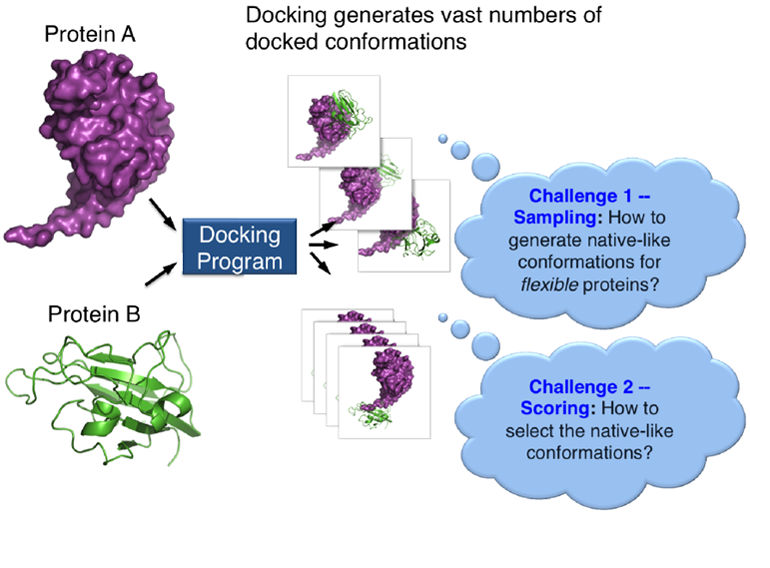
\includegraphics[width=10cm]{imagens/mostra_docking.png}
	\end{figure}
    
Tendo como objetivo analisar e prever a melhor conformidade entre duas estruturas celulares, conhecendo toda a região das moléculas das proteínas, ao aplicar o docking é possível descobrir a afinidade de ligação que estas duas moléculas possuem entre si, sendo assim estimando o melhor encaixe.
Ao ocorrer uma ligação, será liberado uma certa quantidade de energia, esta energia é importante para medir a conformidade da união entre duas moléculas (ligante e receptora).
Para realizar a medição, é utilizado funções de pontuação (score functions), focadas na minimização energética, que  segundo \cite{kitchen2004docking} e \cite{lybrand1995ligand}, chegaram a conclusão de que, quanto menor a energia gasta entre duas moléculas, melhor será sua a conformidade na união. 

Dependendo da estrutura que é analisada com o docking, torna-se possível criar uma substância capaz de inibir a molécula receptora, no caso de um inibidor de vírus por exemplo. \cite{ishikawa2011binding}

Com essa manipulação nas estruturas celulares, é possível destrinchar vários assuntos, pesquisas e artigos sobre os comportamentos de células e proteínas.
Esses exemplos são triviais para o estudo do comportamento das composições químicas das células para fazer medicamentos na área da biomedicina. 
Em geral é a técnica de docking molecular é utilizada para desenvolver estruturas de células diversas; vírus de doenças, medicamentos,DNA e tudo que envolva fármacos. 

Muitos softwares já obtiveram resultados positivos ao utilizar docking, conforme mostrado na tabela 1 abaixo, onde é listado exemplos destes softwares.
\begin{table}[h]
\centering
\caption{Softwares bem sucedidos ao utilizar docking molecular \cite{sliwoski2014computational} }

\begin{tabular}{@{}|c|c|c|@{}}
\toprule

Software & Alvo                   & Estudo                                                   \\ \midrule
Seed     & Plasmepsin             & Uma das causas da malária                                \\ \midrule
FlexX    & Fator de Edema Anthrax & Inibidor do edema                                        \\ \midrule
Glide    & Citocromo P450         & Deixa substâncias em formas hidrosolúveis         \\ \midrule
Surflex  & Topoisomerase I        & Otimização de anti-cancerígeno                           \\ \midrule
Dock     & Imunofilina F506       & Inibidor de calcineurina \\ \bottomrule
\end{tabular}
\end{table}

Para \cite{rodrigues2012estrategias}, o objetivo principal que se tem ao aplicar docking é; aprimorar o processo de busca de novos candidatos a fármacos e acelerar o processo contínuo do seu planejamento. 
Todos os fatores como as propriedades químicas das moléculas auxiliam a compreender de qual maneira se comportará as células, quais os tipos de ligação que podem ser utilizados como; proteína-ligando, proteína-DNA, proteína-proteína. Isso pode influenciar na abordagem de docking e afetar o desempenho nos softwares utilizados, ao serem aplicadas funções de pontuação.

Quanto a abordagem, existem duas formas diferentes de realizar o docking, que pode ser classificado como Docking Rígido e Docking Flexível.

No docking rígido os pontos de união de uma molécula ligante e receptora são mais limitados, isso se deve ao fato de existir uma menor liberdade em manipular as moléculas de uma célula, ou seja, a molécula ligante será rígida assim como o receptor. Consequentemente isso acaba resultando em maiores pontos a serem estimados para realizar a união de uma forma compatível. \\
Isso pode aumentar a precisão de acertos, já que existe vários pontos a serem avaliados e qual deles terá menor energia para realizar o acoplamento \cite{pagadala2017software}. 
Já no Docking Flexível, a molécula ligante pode ser manipulada com total liberdade ao tentar se acoplar no receptor,  este que continuará sendo rígido. O número de pontos a ser estimado será menor por ser ajustado a molécula ligante ao receptor rígido.
Geralmente é utilizado esta abordagem após ser feito o docking rígido, orientado o melhor resultado estimado anteriormente para que desta forma tenha-se uma boa conformidade, isto é ilustrado na figura 2.


      \begin{figure}[!htb]
	\centering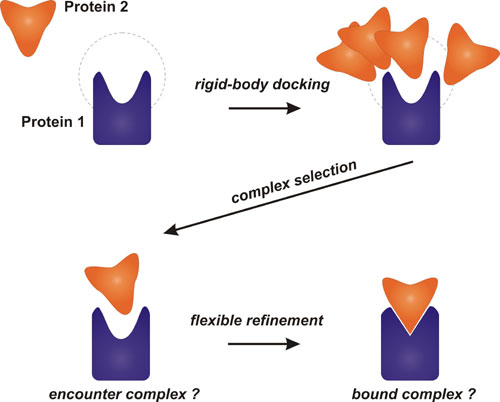
\includegraphics[width=10cm]{imagens/rigid_flexible.jpg}
	\caption{Docking Rígido com refinamento flexível}
	\end{figure}

\section{Função de Pontuação}
O aprendizado de máquina se tornou algo bem comum ao ser aplicado em diversas áreas da computação, ao ser aplicado em software deve ser levantado os pontos que são relevantes para o processo de docking.

Nos softwares de docking são utilizados algoritmos para gerar funções de avaliação para estimar o gasto energético durante a união entre moléculas, como por exemplo algoritmo genético \cite{holland1975adaptation}, Simulate Annealing \cite{kirkpatrick1984optimization} ,  algoritmo genético de Lamarca \cite{morris1998automated},  MonteCarlo \cite{caflisch1992monte}.

Estes algoritmos estão constantemente sendo evoluídos e até substituídos para obterem mais eficácia ao estimar grandes volumes de dados com um desempenho melhor.
Portanto, é possível dizer que ao melhorar a precisão desta função, é possível otimizar o processo de docking molecular consideravelmente.

\section{Software - Autodock Tools e Vina}

Falar um pouco sobre o que é, sobre o que é possível fazer com ele, suas precisões e acertos, mostrando imagens do mesmo.

\section{Técnicas de Aprendizado de Máquina }
%Falar sobre deep learning, svm, florestas aleatorias algoritmo genético e todas ténicas que foram utilizadas anteriormente em softwares
O foco será direcionado para o estudo de uma das técnicas de Inteligência Artificial na literatura, sendo uma delas redes neurais profundas, onde é possível utiliza-la para treinar os algoritmos para previsão e definição dos melhores resultados possíveis. 

Começando pelo pelo básico da IA, temos o aprendizado supervisionado e não supervisionado, dentre estes são utilizados funções de classificação e agregação que são muito limitadas para serem exploradas em um volumes de dados muito grande.
Para estudar o comportamento de uma célula é necessário fazer um mapeamento de sua estrutura para compreender suas peculiaridades e comportamentos. 

Tal processo é muito custoso se tratando do tempo gasto para exibir resultados, dependendo do poder de processamento e da técnica de machine learning utilizada (svm, algoritmo genético random forest). 
Para fazer a máquina explorar e buscar informações referentes a composição das moléculas, será requerido bases de dados (datasets), que irá conter os dados necessários para efetuar treinos e testes. 

Existem diversos softwares que utilizam técnicas de IA, cada um leva em consideração qual aspecto do docking deve ser melhorado. Abaixo é falado sobre alguns desses aspectos.
% \begin{itemize}

\textbf{(1)Poder de Pontuação:} the ability to produce scores for the different binding poses; these scores are supposed to be linearly correlated with the experimentally determined binding affinities of the protein-ligand complexes of known 3D structures. 

\textbf{(2) Poder de Ranqueamento:}
the ability to correctly rank a given set of ligands with known binding poses when bound to a common protein. 

\textbf{(3)Poder de Docking:} the ability to
identify the best binding pose of a given ligand from a set of computationally
generated poses when bound to a specific protein,

\textbf{(4)Poder de escaneamento:}
which is the ability of a scoring function to
identify the true binders to a given target protein among a pool of random
molecules.
% \end{itemize}

%Citar também softwares que utilizam tais técnicas descritas acima

Neste trabalho o foco foi estudar uma otimização do poder de ranqueamento de docking, ou seja, ser capaz de avaliar e estimar qual a melhor estrutura para um determinado ligante ou proteína se encaixar.

Para este caso em específico,\textbf{FULANO} utilizou florestas aleatórias e obteve um resultado satisfatório pois compreende um bom desempenho ao utilizar um grande volumes de parâmetros e  \textbf{BLABLABLA}

\subsection{Random Forests}
Conforme visto na literatura, o desempenho das demais técnicas dependem da performance de execução dos diversos recursos computacionais empregados, ou seja, partindo do pressuposto da utilização da técnica de florestas aleatórias, não será necessários exímios recursos e processamento para melhores resultados, é evidente que quanto mais vezes for treinado e melhor descritos os parâmetros, a eficácia será maior.

Dado o software disposto em GITHUB, foi feito toda sua análise e proposta na sua linguagem nativa C++ com o uso de computação imperativa para estipulação de resultados.

As florestas aleatórias utilizam isso isso e aquilo, do qual é possível criar arquivos com n-features e recursos, para melhor compreendimento de como funcionará as florestas aleatórias, será explicado na seção de metodologia deste trabalho. 

Porém o uso desta técnica pode acarretar o overfiting devido a taltaltal, que pode ser visto a seguir na seção de resultados.

\subsection{Support Vector Machine}

Para que seja considerado a melhor forma de optar por prática em docking foi avaliado os seguintes quesitos:

FALAR DOS REQUISITOS

Para este trabalho foi proposta uma alternativa ao RF-Score, utilizando os mesmos dados porém otimizando os resultados aplicando outra técnica de machine learning, chamada Suporte Vector Machine (svm), com a finalidade de resolver os problemas presentes na implementação de floresta aleatória.

\begin{comment}
\end{comment}

\section{Data-sets}

Falar sobre bases de dados para treino e teste, como dividir e classifica-los. Assim será mais fácil explicar na metodologia

\chapter{Metodologia}
Em primeiro momento o foco será estudar os componentes necessários para realização de docking e  fazer uma revisão bibliográfica dos recursos necessários para realiza-lo.

Esta revisão tem como objetivo se aprofundar nos temas que envolvem todo o processo de docking como onde é aplicado, qual o processo para ser executado, as ferramentas, requisitos necessários  e saber quais os resultados esperados computacionalmente.

A parte de aplicações refere-se ao uso de docking e para o que é útil,  em especial o que seria necessário para desenvolver algum fármaco.

O processo de realizar docking através de softwares ajuda a entender como ocorre o funcionamento desta técnica, com isso é possível saber ter uma estimativa de quais são os requisitos e resultados esperados que serão avaliados computacionalmente.

Após ser estudado o docking foi realizado uma pesquisa a respeito da área de aprendizado de máquina, buscando especificamente o conhecimento da técnica de florestas aleatórias e SVM, que aborda temas como o a classificação das estruturas de proteínas bem como a predição dos melhores pontos estimados do docking.

Também foi feito um levantamento das ferramentas existentes; de quais ferramentas (softwares) são utilizados e quais foram as otimizações das funções de avaliação que tiveram ao longo dos anos segundo os benchmarks.

Assim como também testar e utilizar softwares,bases de dados, api's e frameworks de linguagens de programação, especificamente o módulo sklearn (CITAR DOCUMENTACAO)do Python que auxiliem no desenvolvimento e treino do aprendizado de máquina.

\section{Materiais Utilizados para Avaliação}
É necessário baixar bases de dados em formatos de arquivo .pdb, que podem ser baixadas através do site (PDBBind). Essas bases contêm todas as informações necessárias para conhecer a estrutura das proteínas, ligantes e DNA. 
O uso dessas bases será de extrema importância,pois ao utiliza-la será possível aplicar treinamento e com isso estimar resultados no ao realizar um teste. 
Os dados das bases irão conter informações referentes de cada molécula, ou seja, parâmetros de afinidade (pdbaff, distância euclidiana, PDB. Mais para frente será comentado sobre a importância desses aspectos.

No arquivo .pdb será utilizado para treino informações relevantes sobre: 
\begin{itemize}

\item \textbf{Posição:} Coordenadas x,y,z;
\item \textbf{Ordem:} 4
\item \textbf{Nome:} C11
\item \textbf{Propriedade Química} : C (representa carbono)

\end{itemize}

Esse arquivo pode ser aberto no software AutoDock, utilizando o pdt (protein docking tools) para manipular a estrutura, adicionar ligantes e parâmetros extras, remoção de átomos de água, escolher pontos para simulação de interações, otimização e desenvolvimento de proteínas. 

Após ser executado o processo desejado é salvo em um formato pdbqt que será lido pelo software vina. Este é encarregado de calcular e estimar os melhores pontos de interação para ser realizado o docking, que exibe em Kcal dos 3 melhores resultados.

Este é o procedimento utilizado pelos cientistas e biotecnologos ao utilizar estas ferramentas, logo após ser feita a triagem simulada é escolhido pelos especialistas os melhores resultados estimados pelo Vina e assim feita a triagem em vitro, onde é tirada a prova real da qualidade das ligações.

Uma excelente métrica que diversos pesquisadores utilizam para testes e avaliaçõe, é através do cálculo de coeficiente de correlação de Pearson e o desvio de raiz quadrada médio (RMSE), este último especificamente para erro, pois é possível comparar o overfiting no treinamento e teste.

\section{Definição de Parâmetros}

Explicar sobre os labels e parâmetros utilizados para teste e treino do SVM.
O que são as afinidades (pdbaff), distância euclidiana (6.6,6.7) e qual label (PDB) utilizado.

\section{Bibliotecas e API's Sklearn do Python}

Falar de quais módulos, bibliotecas e funções  foram utilizados.

\chapter{Resultados}

\section{Resultados do Random Forest}

No trabalho proposto por \textbf{BALLESTER} foi obtido os seguintes resultados:

Mostrar imagem e gráficos do artigo dele.

\section{Resultados do SVM}

Ao utilizar svm como alternativa foi possível obter tais resultados:

Mostrar o resultado que obtive com imagens e gráficos.

\section{SVM X Random Forest}

Ao utilizar a técnica de Random Forest o resultado de tal e tal é bom para tal coisa mas isso leva uma má impressão de outra coisa, que no SVM deixa o resultado mais evidente pois tal tal tal.

\chapter{Conclusões}

Colocar toda análise de cada capítulo aqui desde a introdução,fundamentação teórica,metodologia e resultados.

\section{Trabalhos Futuros}

Falar na conclusão ou deixar separado.

\bibliography{relatorio}
\bibliographystyle{abnt}

%\appendix

\end{document}

